\section{最小绝对值回归性能优化}

\begin{frame}{交替凸优化算法的计算性能问题}
    \begin{itemize}
        \item
        交替凸优化算法需要求解多个最小绝对值回归问题,
        在变量较多情况下,线性规划算法计算性能较差。
    \end{itemize}
\begin{figure}[H]
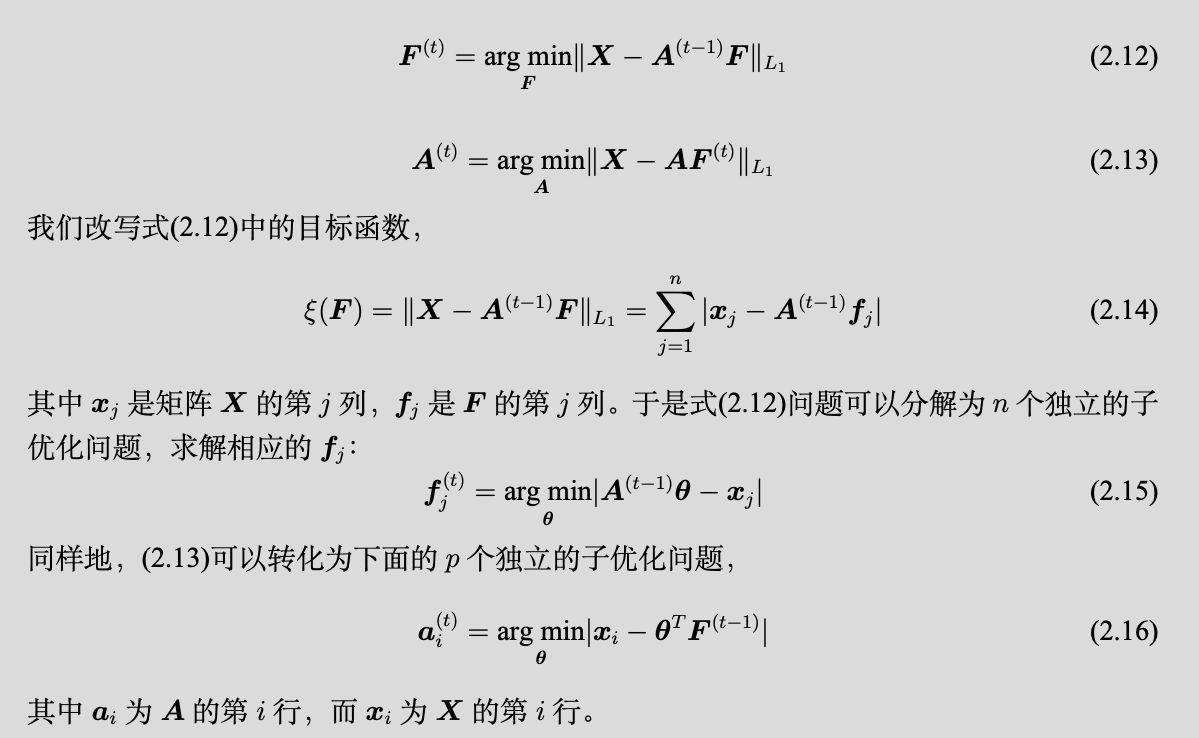
\includegraphics[width=8cm]{pics/acp-problem.png}
\end{figure}
\end{frame}

\begin{frame}{最小绝对值回归的优化1: 聚类——迭代拆解算法}
    \begin{itemize}
        \item
        Park等人于2016年提出一种聚类——迭代拆解算法,通过减小问题规模来提升计算性能。
    \end{itemize}
    \begin{figure}[H]
        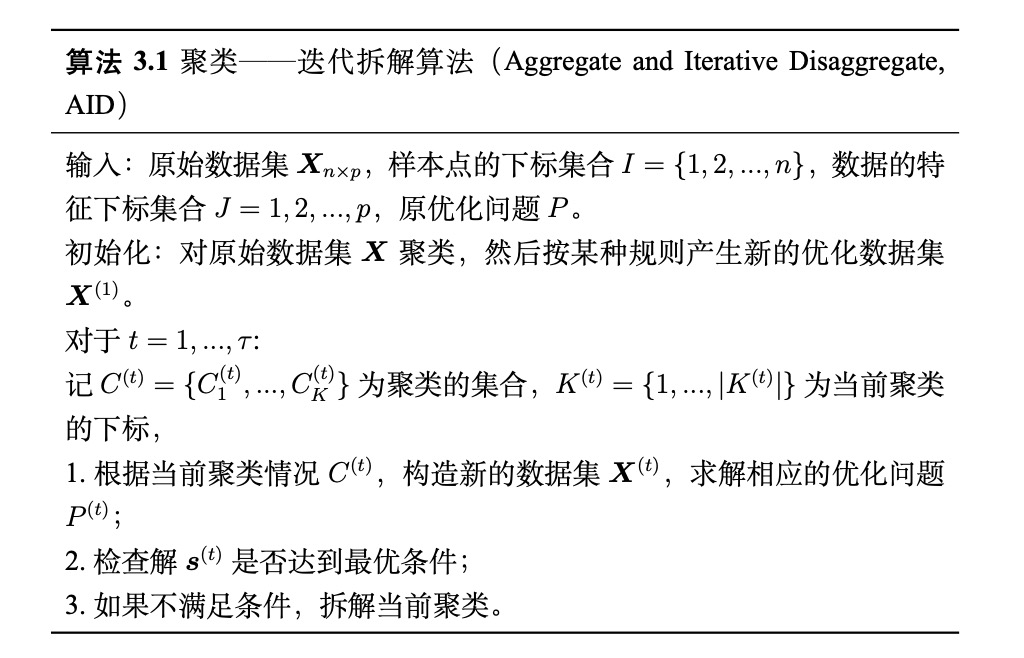
\includegraphics[width=10cm]{pics/aid-al.png}
    \end{figure}
\end{frame}
\begin{frame}{最小绝对值回归的优化1: 聚类——迭代拆解算法}
    \begin{itemize}
        \item 初始聚类,使用任意聚类方法,我们这里使用K-means。
    \end{itemize}
\begin{figure}[H]
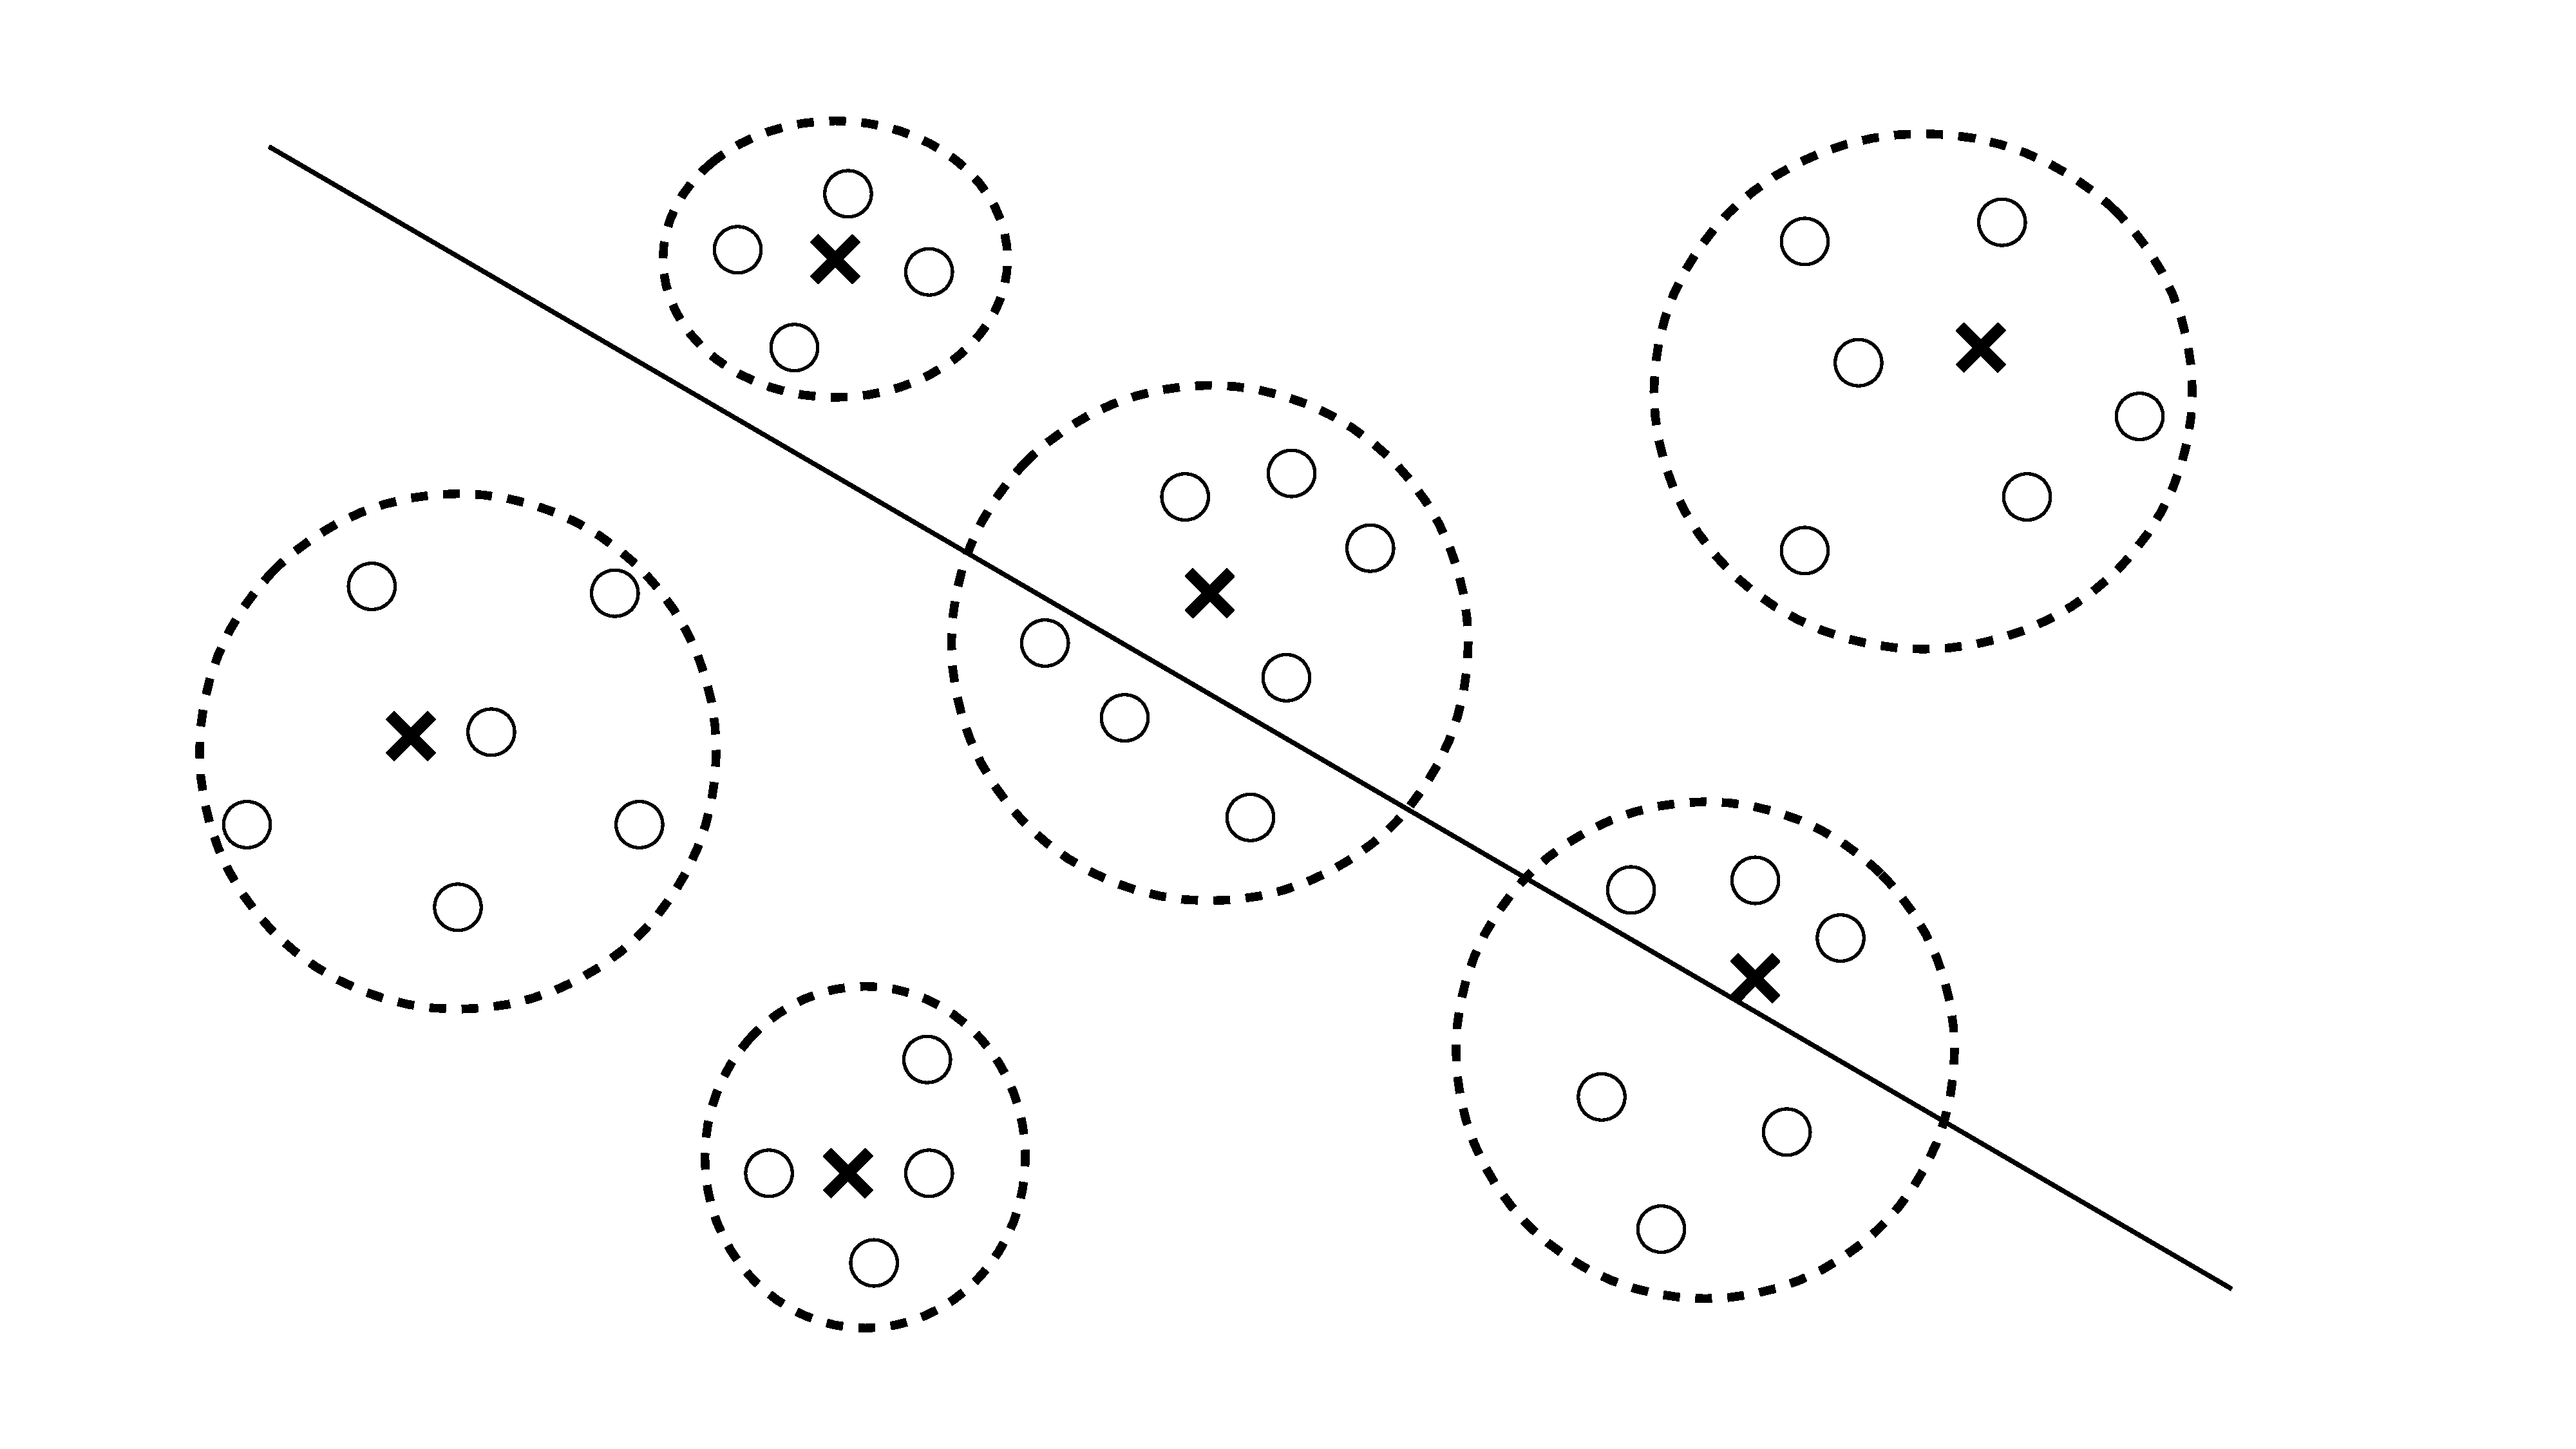
\includegraphics[width=10cm]{pics/aid-demo-a.pdf}
\end{figure}
\end{frame}

\begin{frame}{最小绝对值回归的优化1: 聚类——迭代拆解算法}
    \begin{itemize}
        \item 计算$\bm \beta$,按规则对聚类进行拆解。
    \end{itemize}
\begin{figure}[H]
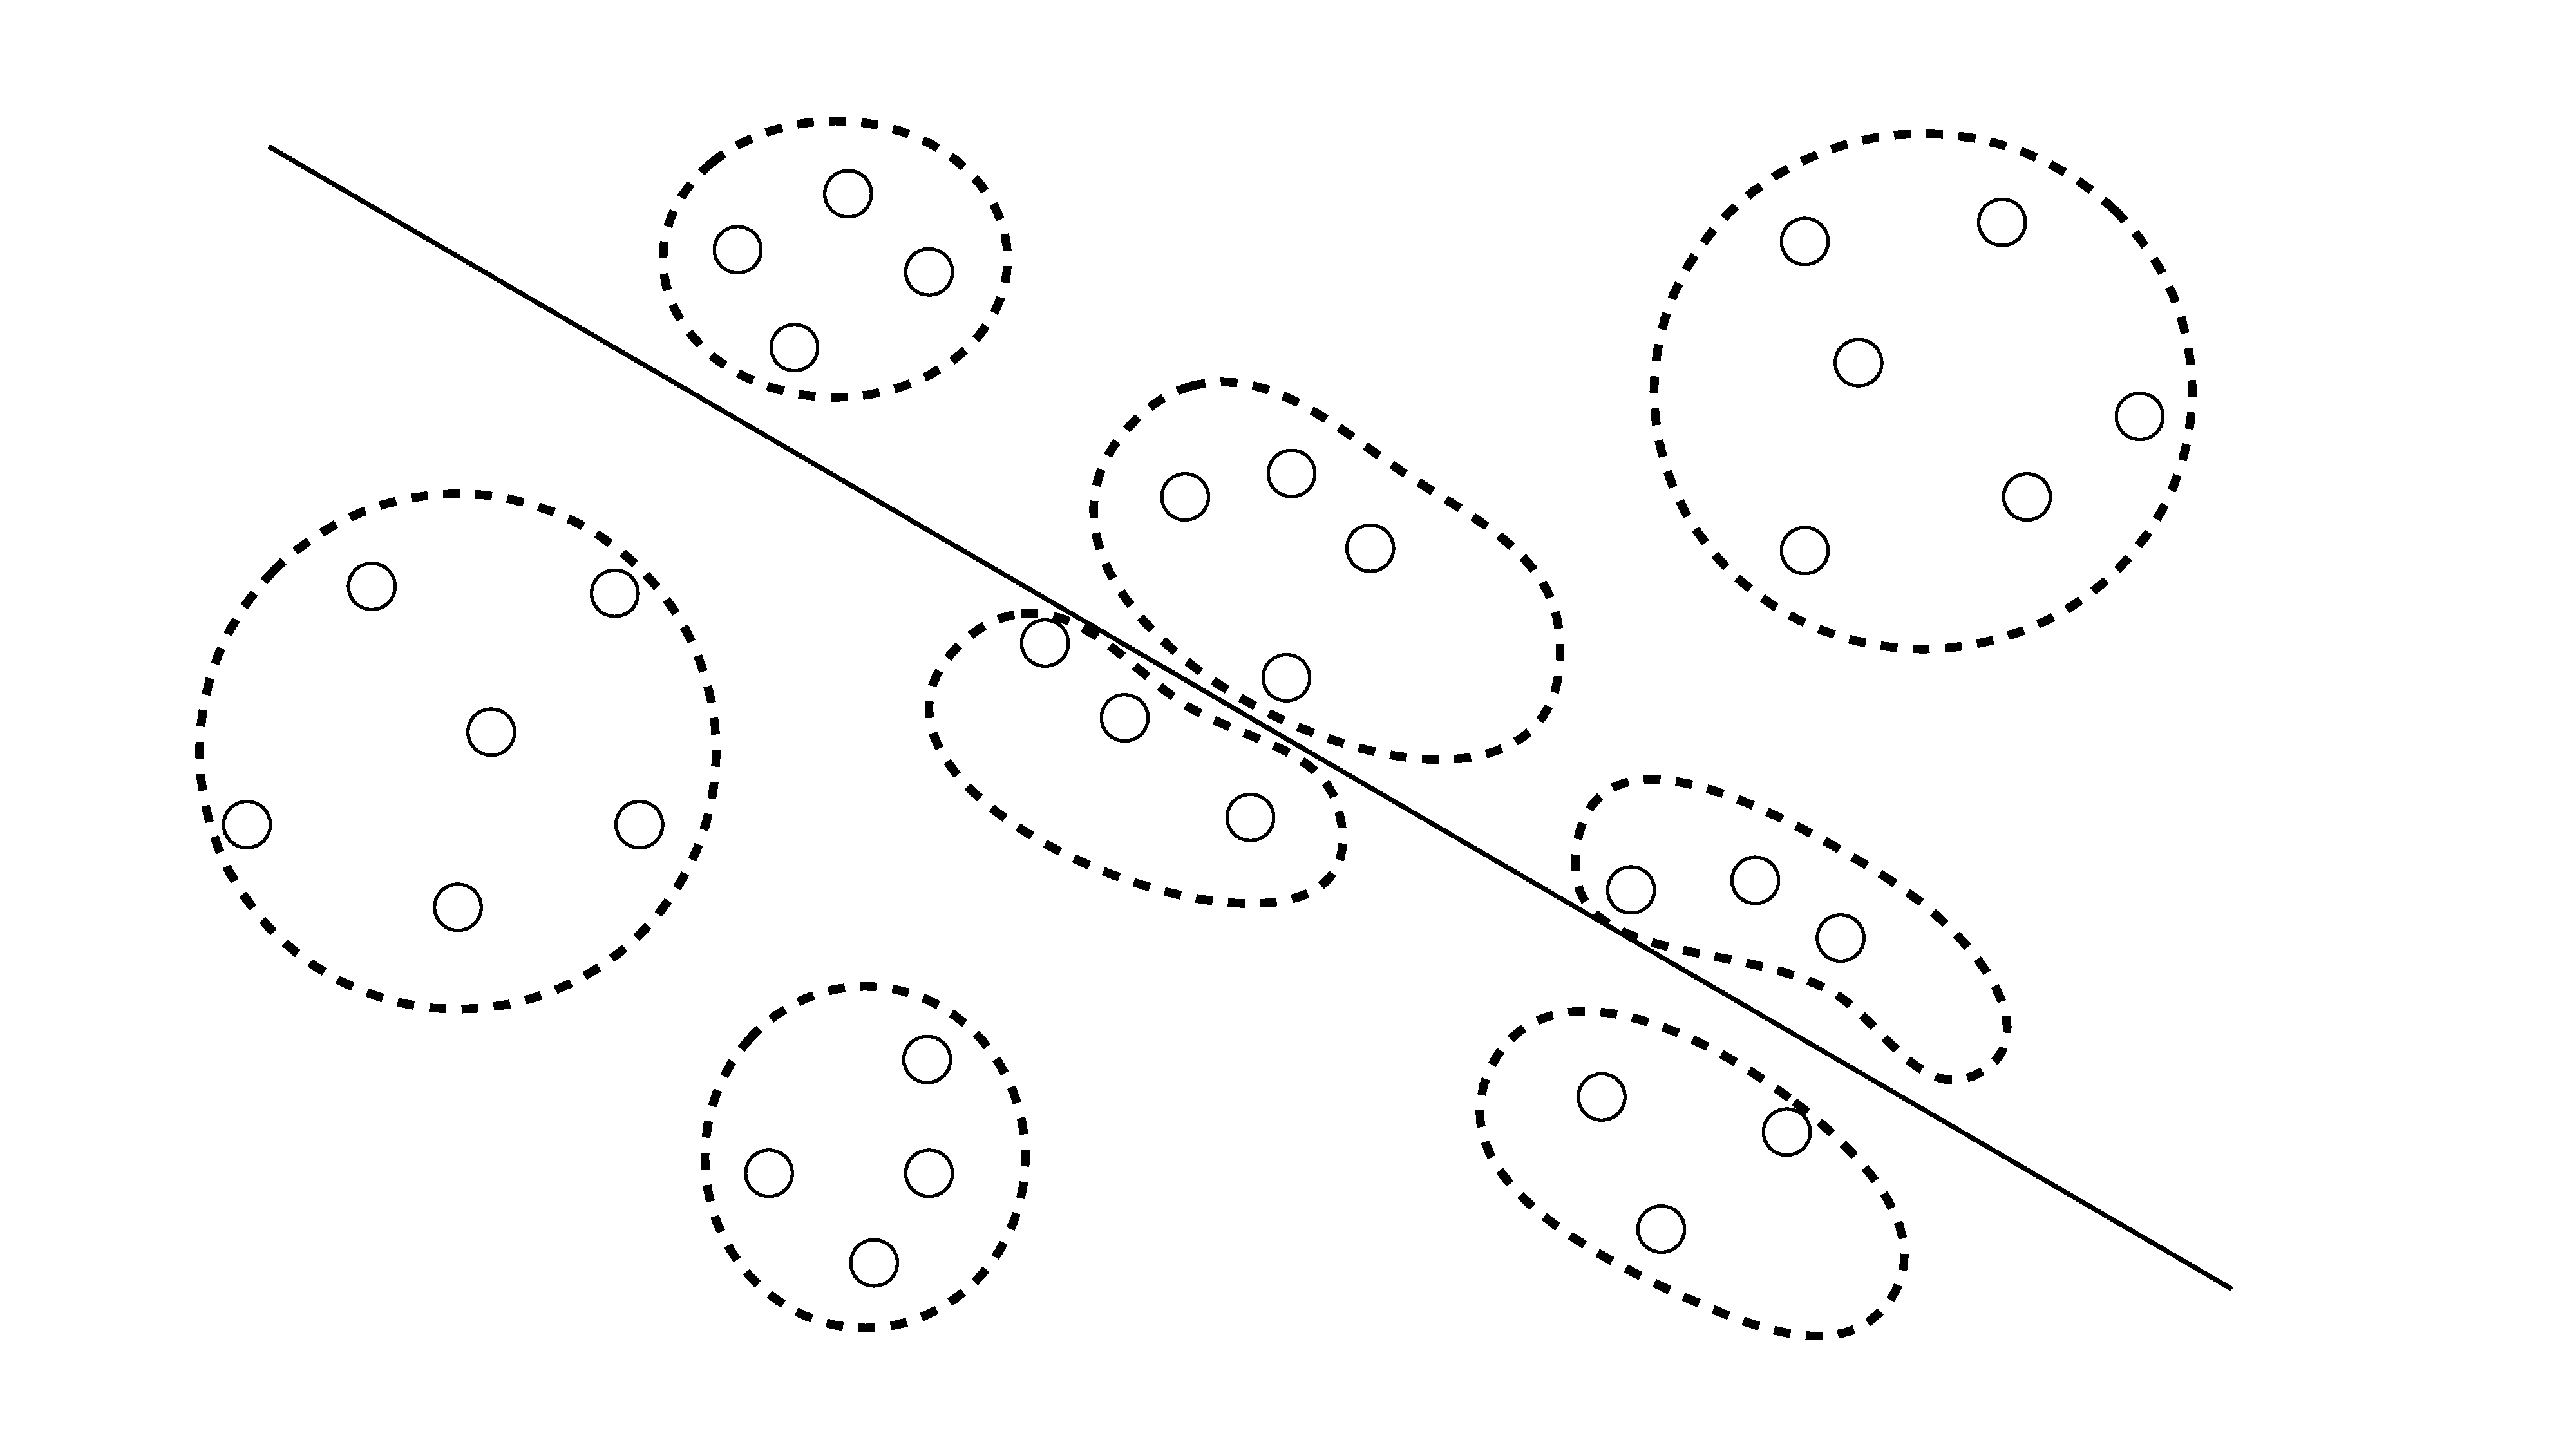
\includegraphics[width=10cm]{pics/aid-demo-b.pdf}
\end{figure}
\end{frame}

\begin{frame}{最小绝对值回归的优化1: 聚类——迭代拆解算法}
    \begin{itemize}
        \item 在新的聚类上重新计算$\bm \beta$。
    \end{itemize}
\begin{figure}[H]
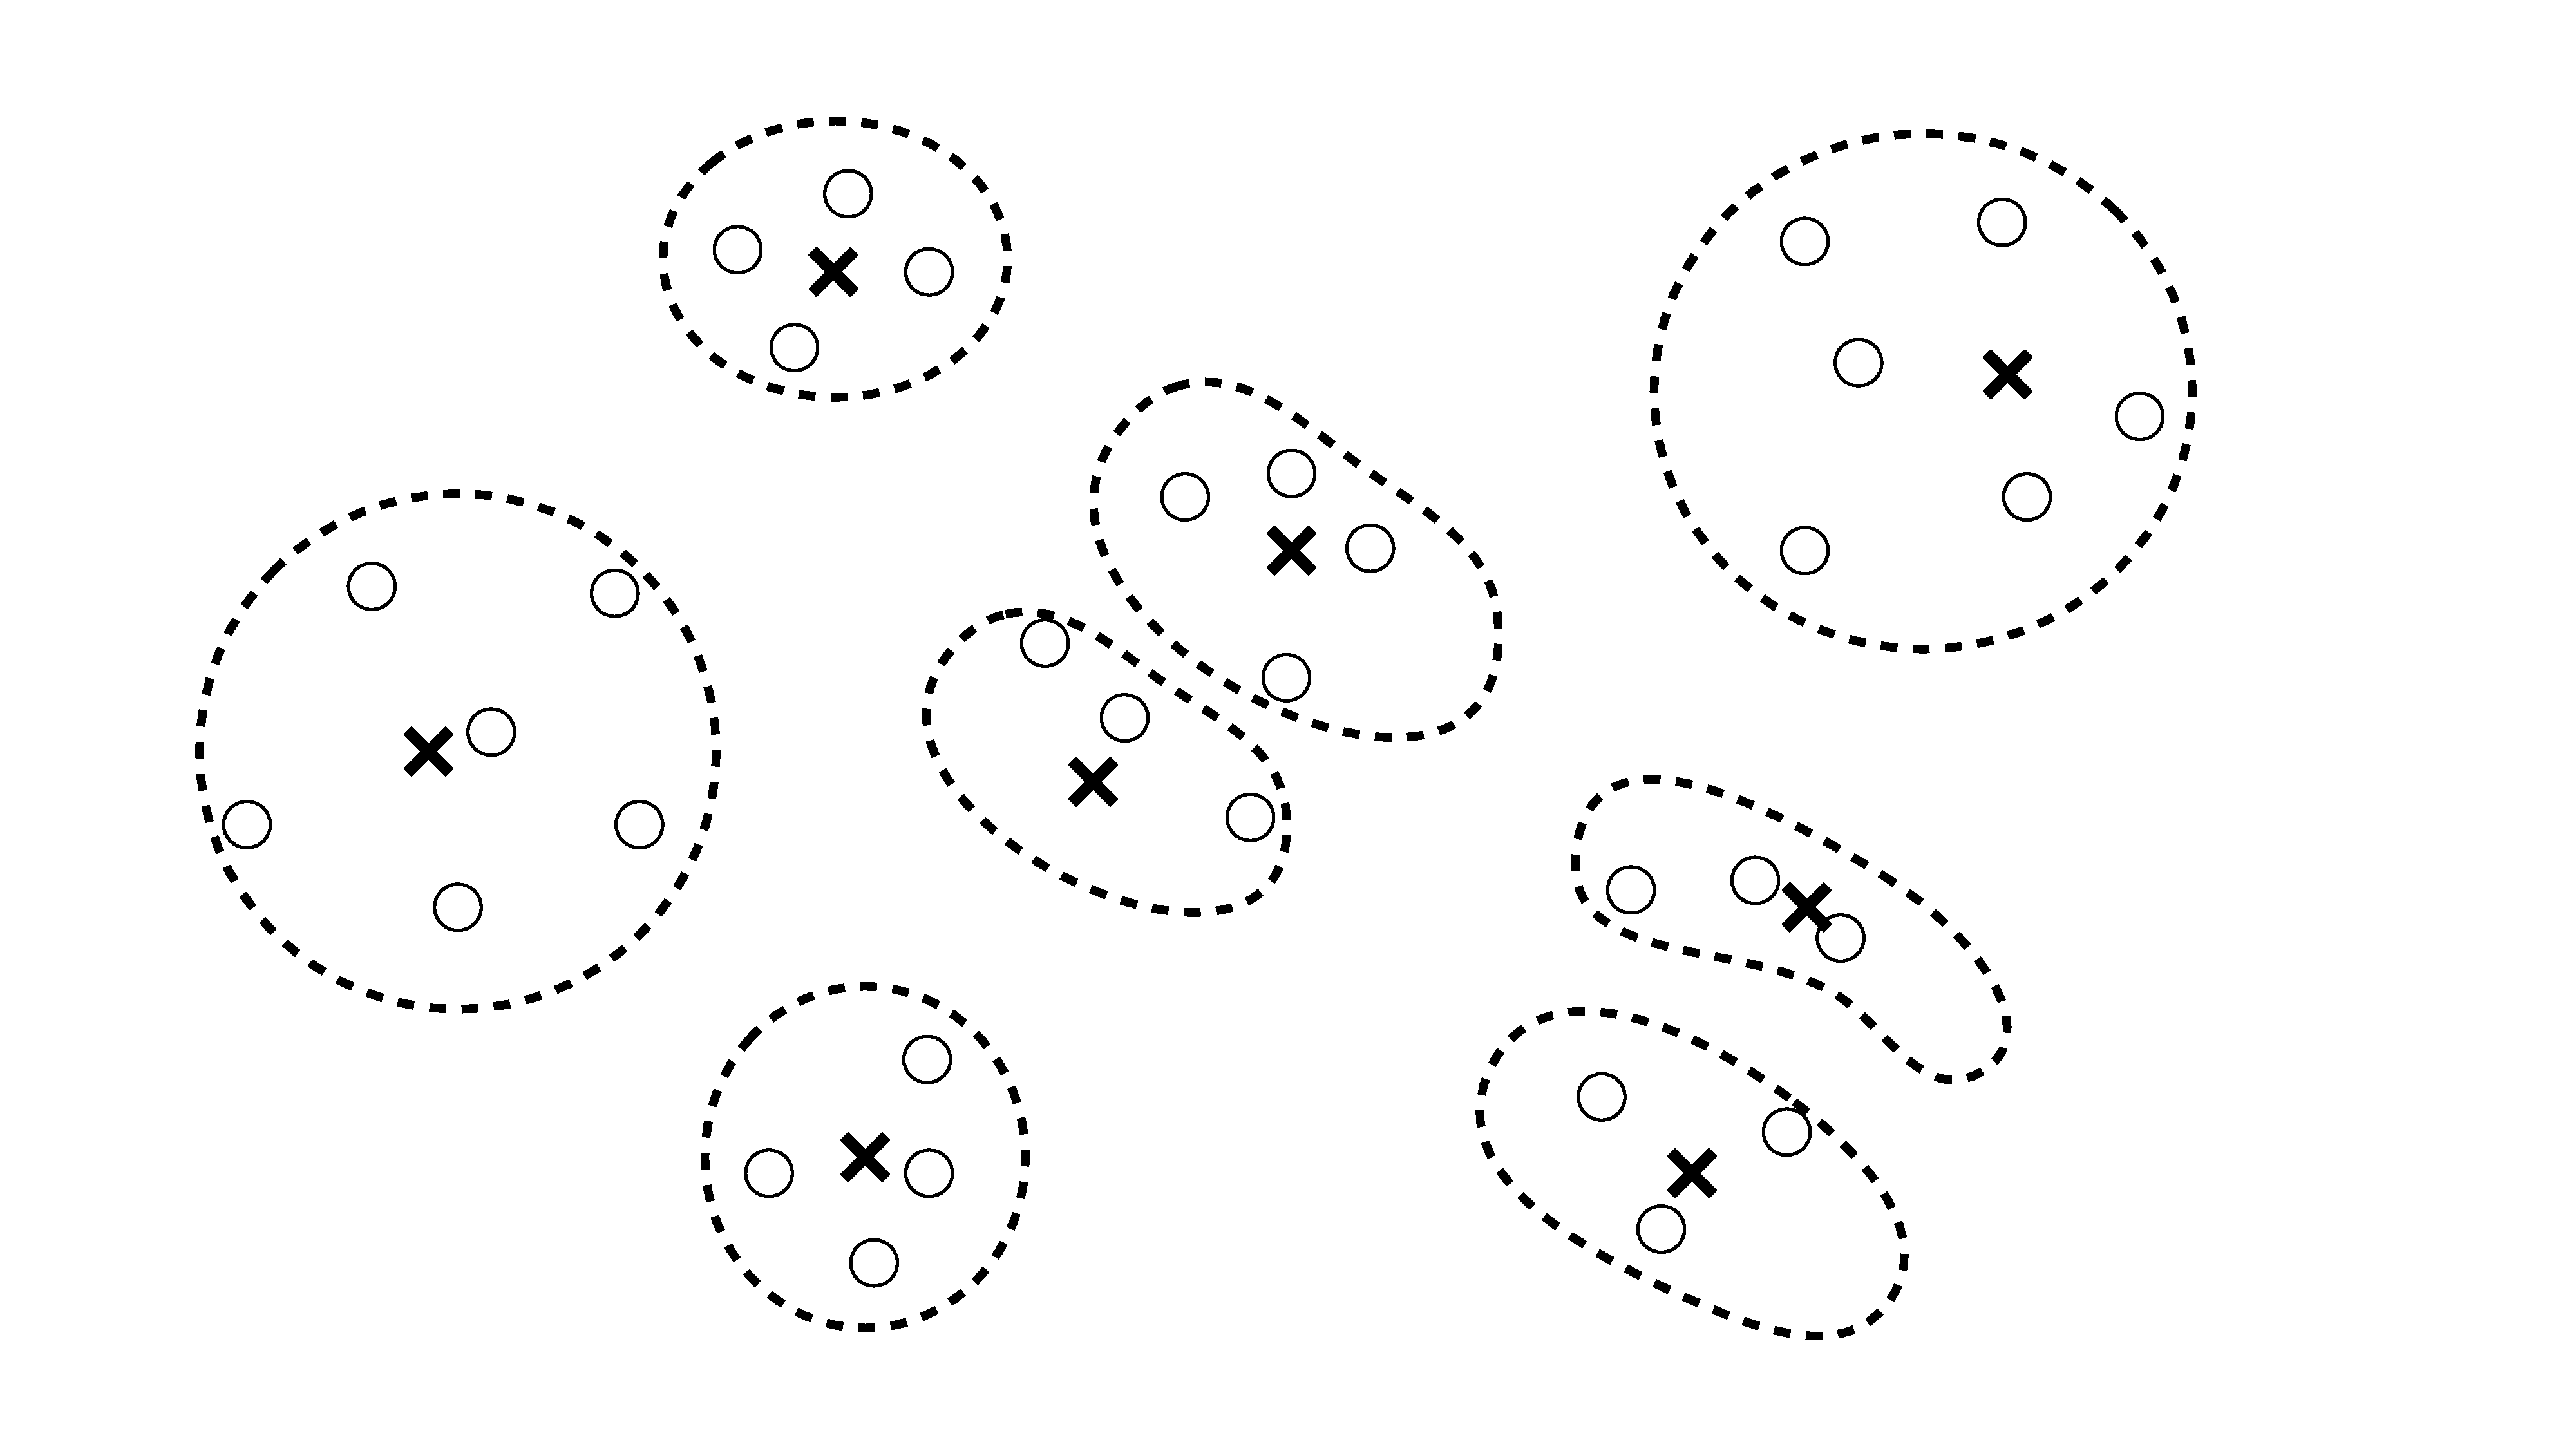
\includegraphics[width=10cm]{pics/aid-demo-c.pdf}
\end{figure}
\end{frame}

\begin{frame}{最小绝对值回归的优化1: 聚类——迭代拆解算法}
    \begin{itemize}
        \item 可以证明,该方法最终获得原问题的最优解
        (和在全部数据上解原优化问题有相同的解)。
    \end{itemize}
\begin{figure}[H]
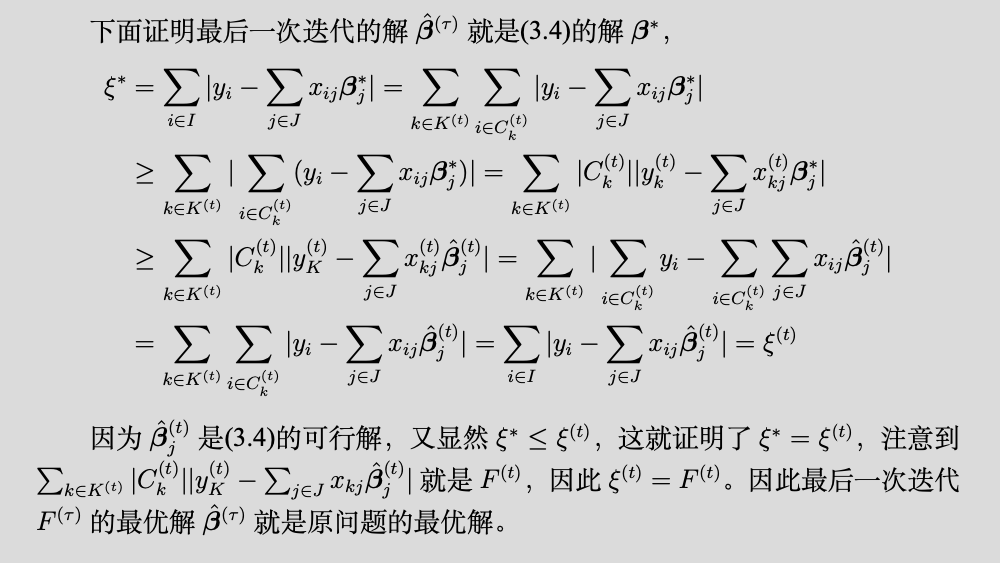
\includegraphics[width=10cm]{pics/proof-aid.png}
\end{figure}
\end{frame}

\begin{frame}{最小绝对值回归的优化2: 基于替代变量的估计算法}
    \begin{itemize}
        \item Weidong Liu等人于2020年提出了一种基于替代变量的估计方法。
        \item 该方法可以优化一般的分位数回归问题,最小绝对值回归就是
        中位数回归,因此我们针对该特例给出步骤和推导。
        \item 这是一种拟牛顿法。该方法利用替代变量,转化为最小二乘问
        题,简化计算。
    \end{itemize}
\end{frame}

\begin{frame}{最小绝对值回归的优化2: 基于替代变量的估计算法}
    \begin{itemize}
        \item 从牛顿-拉弗森迭代出发,对问题进行探究。
    \end{itemize}
\begin{figure}[H]
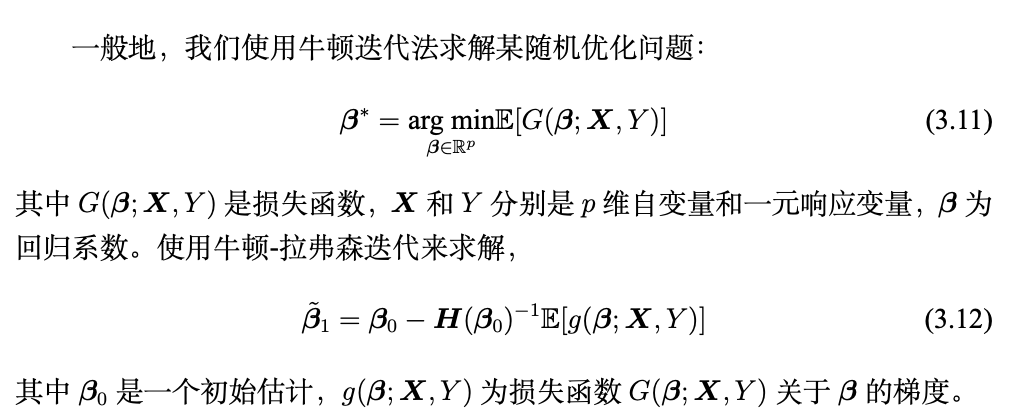
\includegraphics[width=10cm]{pics/step1.png}
\end{figure}
\end{frame}

\begin{frame}{最小绝对值回归的优化2: 基于替代变量的估计算法}
    \begin{itemize}
        \item 当$\bm \beta_0$和$\bm \beta^*$十分接近时,可以做一点近似。
    \end{itemize}
\begin{figure}[H]
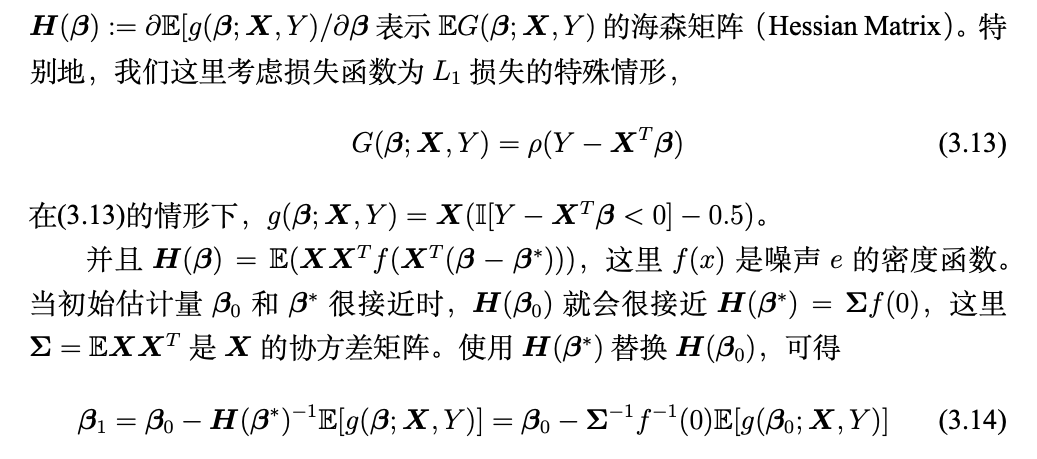
\includegraphics[width=10cm]{pics/step2.png}
\end{figure}
\end{frame}

\begin{frame}{最小绝对值回归的优化2: 基于替代变量的估计算法}
    \begin{itemize}
        \item 在这种近似下,牛顿迭代依然可以逼近最优解。
    \end{itemize}
\begin{figure}[H]
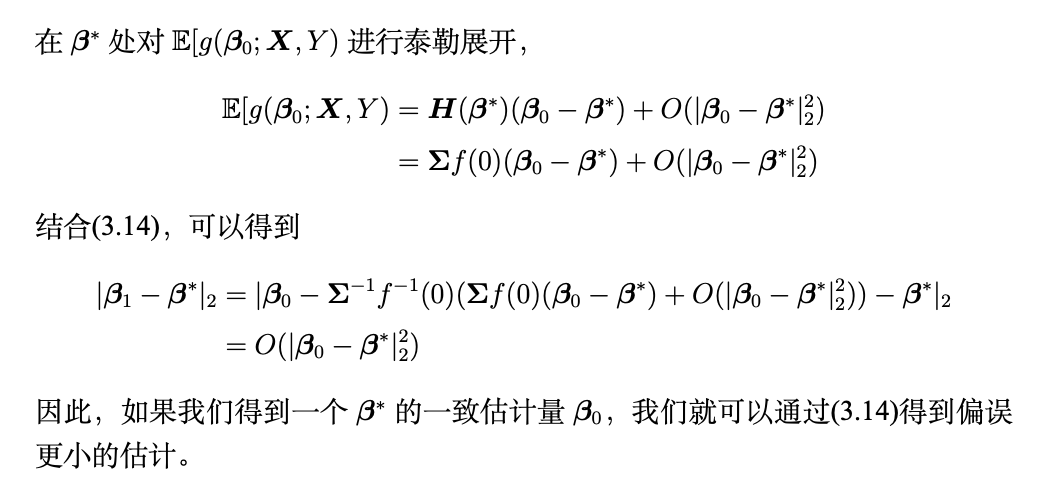
\includegraphics[width=10cm]{pics/step3.png}
\end{figure}
\end{frame}

\begin{frame}{最小绝对值回归的优化2: 基于替代变量的估计算法}
    \begin{itemize}
        \item 利用替代变量,转化为一个最小二乘问题。
    \end{itemize}
    \small
    \begin{equation}
        \begin{split}
        \bm{\beta}_1 &= \bm{\Sigma}^{-1}(\bm{\Sigma}\bm{\beta}_0 - f^{-1}(0)\mathbb{E}[g(\bm{\beta}_0;\bm{X},Y)])\\
        &= \bm{\Sigma}^{-1}\mathbb{E}[\bm{X}\{\bm{X}^T\bm{\beta}_0 - f^{-1}(0)(\mathbb{I}[Y \leq \bm{X}^T\bm{\beta}_0] - 0.5)\}]
        \end{split}
    \end{equation}
    这里我们定义一个新的响应变量$\tilde Y$,
    \begin{equation}
        \tilde Y = \bm{X}^T\bm{\beta}_0 - f^{-1}(0) (\mathbb{I}[Y \leq \bm{X}^T\bm{\beta}_0] - 0.5)
    \end{equation}
    那么$\bm{\beta}_1 = \bm{\Sigma}^{-1}\mathbb{E}(\bm{X}\tilde{Y})$就是线性回归问题$\tilde Y = \bm{X}^T\bm{\beta}$
    的最优回归系数,即
    \begin{equation}\label{beta1-original}
        \bm{\beta}_1 = \underset{\bm{\beta} \in \mathbb{R}^{p}}{\operatorname{arg\ min}} 
        \mathbb{E}(\tilde Y - \bm{X}^T \bm{\beta})^2
    \end{equation}
\end{frame}

\begin{frame}{最小绝对值回归的优化2: 基于替代变量的估计算法}
    \begin{table}[H]%%%%%%开始表格
        \centering%把表居中
        \tiny
        \begin{tabular}{{p{0.9\columnwidth}}}%三个c代表该表一共三列,内容全部居中
        
        \toprule%第一道横线 表头
         使用替代变量迭代算法方法求解最小绝对值回归问题(SVN, Substitue Variable Newton method)\\
        \midrule%第二道横线 符号+解释+单位 中间用&隔开
        输入:$Y$和$\bm{X}$的样本$\bm{Y} = (Y_1, Y_2, ..., Y_n)$,$\bm{X} = (\bm{X}^{\rm T}_1, \bm{X}^T_2, ..., \bm{X}^T_n)$,
        迭代次数$\tau$,核函数$K(x)$,依赖于迭代次数的带宽$h^{(t)}$,
        $(t = 1, ..., \tau)$。
        \\
        初始化:给出初始相合估计量$\hat{\bm{\beta}}^{0} $,将样本划分成$J$个均等子集,样本量均为$m$,为了给出最小绝对值回归估计量的相合估计,
        我们取任一子集里面的数据,直接使用最小一乘法估计$\hat{\bm{\beta}}^{0}$。
        \\
        对于$t = 1, ..., \tau$:
        取新的数据子集,在该数据集上
        \\
            1. 计算$\hat{f}^{(t)}(0)$,
            $$
            \hat{f}^{(t)}(0) = \frac1{mh}\sum_{i=1}^{m}K(\frac{Y_i - \bm{X}_i^T\hat{\bm{\beta}}^{(t-1)}}{h^{(t)}})
            $$
        \\
            2. 计算$\tilde{Y} = (\tilde Y_1, \tilde Y_2, ..., \tilde Y_m)$,
            $$
            \tilde{Y}_i = \bm{X}^T_i\hat{\bm{\beta}}^{(t-1)} - \hat{f}^{(t)}(0)^{-1}
            (\mathbb{I}[Y_i \leq \bm{X}_i^T \hat{\bm{\beta}}^{(t-1)}] - 0.5)
            $$
        \\
            3. 计算$\hat{\bm{\beta}}^{(t)}$,
            $$
            \hat{\bm{\beta}}^{(t)} = \underset{\bm{\beta} \in \mathbb{R}^{p}}{\operatorname{art\ min}}
            \frac1{m}\sum_{i=1}^m (\tilde{Y}_i - \bm{X}_i^T\bm{\beta})^2
            $$
        \\
        输出:$\hat{\bm{\beta}}^{(\tau)}$
        \\
        \bottomrule%第三道横线
        \end{tabular}
    \end{table}%%%%%%结束表格
    
\end{frame}

\begin{frame}{算法的性能比较实验}
    \begin{itemize}
        \item 利用模拟数据,观察和测试算法的运算性能。
        \item SVN算法为拟牛顿法,这里先比较不设置终止条件下的结果。
    \end{itemize}

    \begin{table}[H]
        \tiny
        \caption{\small 高斯噪声下三种估计算法的性能比较}
        \label{tab-performance}
        \centering
        \begin{tabular}{@{}ccccccccc@{}}
        \toprule
               &     & \multicolumn{4}{c}{AID}        & \multicolumn{2}{c}{SVN} & LP        \\ \midrule
        n      & p   & $r^0$(\%) & $r^\tau$(\%) & $\tau$  & Time(sec) & $\tau$      & Time(sec)      & Time(sec) \\ \midrule
        20000  & 10  & 0.05  & 2.90  & 6  & 2         &  3      &         0.38       & 0.20      \\
        20000  & 50 & 0.15  & 12.00 & 12 & 13        &   7     &          6     & 3       \\
        20000  & 100 & 0.15  & 12.00 & 12 & 38        &  11      &         27    & 21         \\
        20000  & 200 & 0.66  & 21.55 & 9  & 118        &   8     &          76      & 126        \\
        20000  & 500 & 0.80  & 28.00 & 11 &  535      &  3      &              322  &     813 \\ 
        40000  & 10  & 0.05  & 2.90  & 6  & 3        &  3      &         0.74      & 0.23     \\
        40000  & 50 & 0.15  & 12.00 & 12 & 31        &   7     &          14     & 7       \\
        40000  & 100 & 0.15  & 12.00 & 12 & 84       &  8      &         56    & 48         \\
        40000  & 200 & 0.66  & 21.55 & 9  & 210        &   8     &          154     & 258        \\
        40000  & 500 & 0.80  & 28.00 & 11 & 1965       &  3      &             1143   &  3446      \\ 
        200000  & 100 & 0.80  & 11.00 & 11 & 134       &  3      &          361      &   496     \\ 
        200000  & 200 & 0.80  & 28.00 & 11 & 2476       &  3      &          1631      &   3329     \\ 
        \bottomrule
        \end{tabular}
    \end{table}
\end{frame}

\begin{frame}{算法的性能比较实验}
    \begin{itemize}
        \item 比较SVN算法设置终止条件下的结果。
    \end{itemize}

    \begin{table}[H]
        \small
        \caption{部分性能结果对比}\label{perfomance2}
        \resizebox{\textwidth}{!}{
        \begin{tabular}{@{}ccccccccccc@{}}
            \toprule
            s & n     & p   & $\tau$ & Time(SVN) & Time(SVN-full) & Time(LP) & Time(AID) & $l_2$-error(SVN) & $l_2$-error(LS) & $l_2$-error(LP) \\ \midrule
            5 & 20000 & 10  & 12        & 0.12      & 0.42           & 0.17     & 2         & 0.0023        & 0.7304       & 0.0024       \\
            5 & 20000 & 50  & 8         & 1         & 7              & 3        & 13        & 0.0039        & 3.1548       & 0.0020       \\
            5 & 20000 & 100 & 14        & 10        & 28             & 19       & 41        & 0.0059        & 15.0373      & 0.0033       \\
            5 & 20000 & 200 & 27        & 81        & 130            & 170      & 124       & 0.0188        & 151.4039     & 0.0028       \\ 
            5 & 20000 & 500 & 40        & 437        & 437             & 1119       & 698        & 0.0259        & 245.0070      & 0.0026       \\
            \bottomrule
            \end{tabular}
        }
    \end{table}
\end{frame}

\begin{frame}{算法的性能比较实验}
    \begin{itemize}
        \item 观察SVN算法的收敛性
    \end{itemize}
    $$
    h^{(t)} = \sqrt{\frac{s\log n}{n}} + s^{-1/2} (\frac{s^2\log n}{10m})^{(t+1)/2},
    $$
    \begin{figure}[H]
        \centering
        \begin{subfigure}[t]{0.3\textwidth}\label{svn-demo1}
        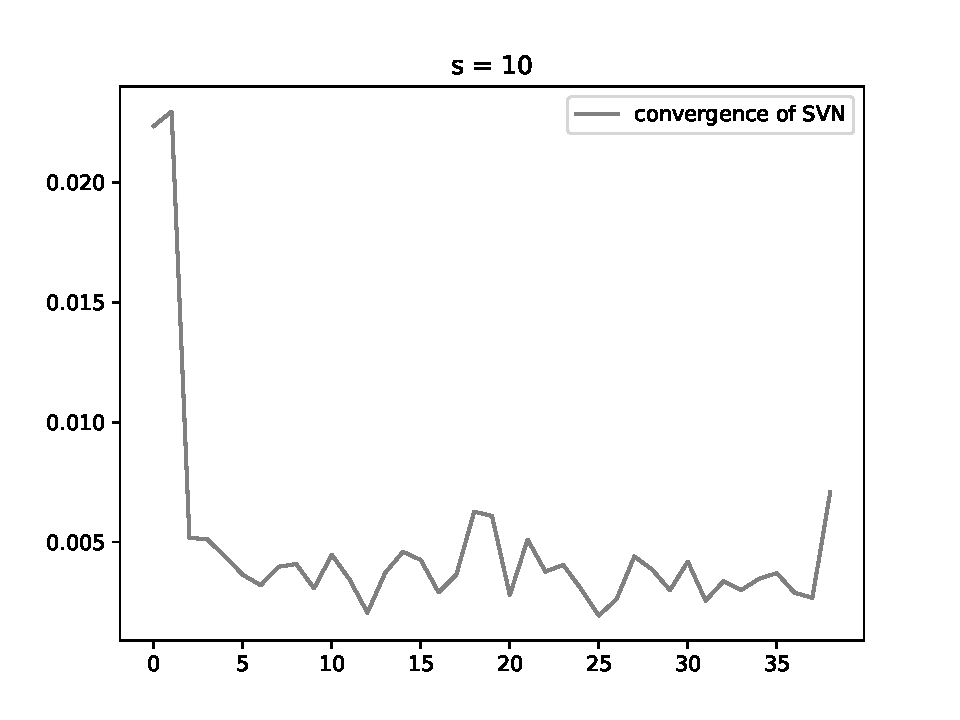
\includegraphics[width=3.9cm]{pics/svn-con-1.pdf}
        \captionof{figure}{}
        \end{subfigure}
        \begin{subfigure}[t]{0.3\textwidth}\label{svn-demo2}
        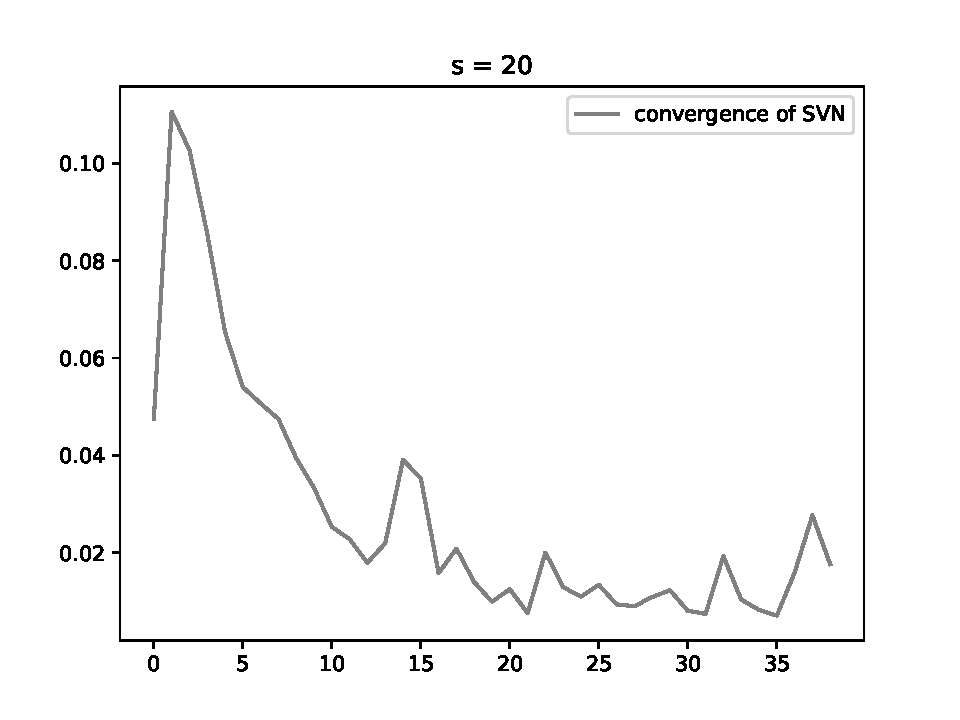
\includegraphics[width=3.9cm]{pics/svn-con-2.pdf}
        \captionof{figure}{}
        \end{subfigure}
        \begin{subfigure}[t]{0.3\textwidth}\label{svn-demo3}
        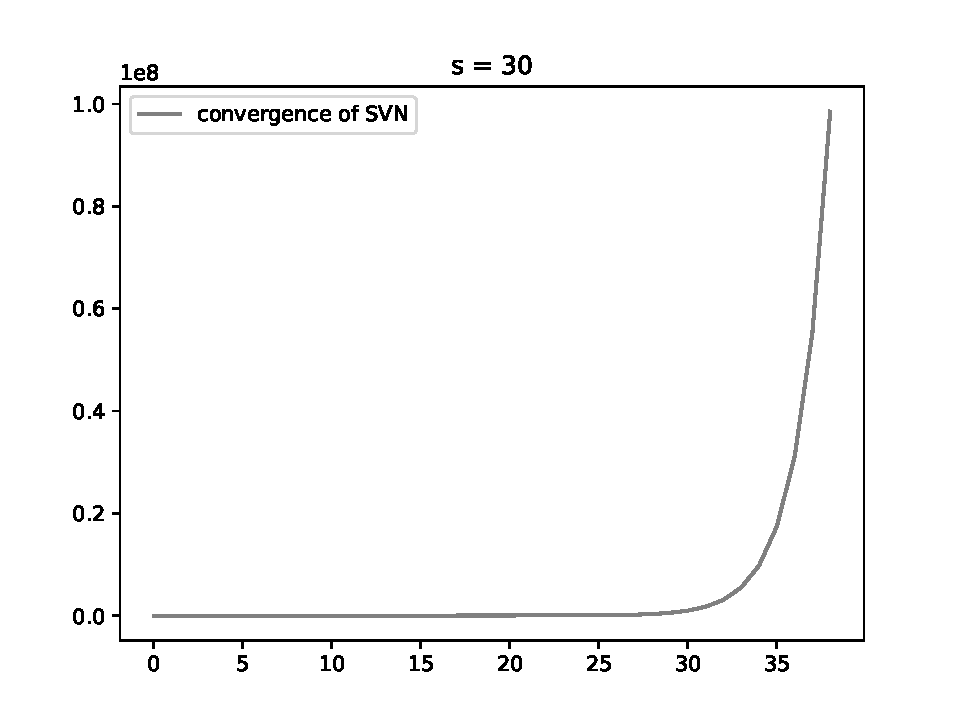
\includegraphics[width=3.9cm]{pics/svn-con-3.pdf}
        \captionof{figure}{}
        \end{subfigure}
        \caption{ \small SVN算法的收敛情况}
        \label{svn-demo}
    \end{figure}
\end{frame}

\begin{frame}{算法的性能比较实验—总结}
    \begin{itemize}
        \item SVN算法在计算性能上很有优势。 
        \item SVN算法作为拟牛顿法不能保证最终收敛到最优解。
        可以设置适当的终止条件。
        \item AID算法最后获得与对全部数据求线性规划相同的解,
        它在数据量较大时也有计算性能的优势。
    \end{itemize}
\end{frame}

\begin{frame}{改进交替凸优化算法}
    \begin{itemize}
        \item 可利用SVN算法改进交替凸优化算法。
        \item 可利用AID算法改进交替凸优化算法。
    \end{itemize} 
\end{frame}

\begin{frame}{改进交替凸优化算法—模拟实验}
    \begin{itemize}
        \item 产生一个服从因子模型的模拟数据集。
        \item 比较ACP-LP,ACP-SVN,ACP-AID的计算时间和重构误差中位数。
    \end{itemize} 
    \begin{table}[H]
        \tiny
        \centering
        \caption{三种算法的比较结果}
        \label{three-l1-pca}
        \begin{tabular}{@{}cccccccccc@{}}
        \toprule
           &      &     & \multicolumn{2}{c}{ACP} & \multicolumn{2}{c}{ACP-SVN} & \multicolumn{2}{c}{ACP-AID} & PCA-L2   \\ \midrule
        m  & n    & p   & Time     & l2-error     & Time       & l2-error       & Time       & l2-error       & l2-error \\ \midrule
        5  & 1000  & 50  & 47       & 0.0083       & 19         & 0.0115         & 129        & 0.0083         & 0.39     \\
        10 & 1000  & 50  & 68       & 0.0064       & 17         & 0.0096         & 104        & 0.0064         & 0.58     \\
        5  & 5000 & 50  & 119      & 0.0382       & 31         & 0.1232         & 278        & 0.0382         & 1.24     \\
        10 & 5000 & 50  & 107      & 0.0259       & 79         & 0.1352         & 321        & 0.0259         & 0.85     \\
        5  & 5000 & 100 & 689      & 0.0725       & 362        & 0.1480         & 1782       & 0.0725         & 1.26     \\
        10 & 5000 & 100 & 792      & 0.0664       & 510        & 0.2394         & 1440       & 0.0664         & 2.99     \\
        5  & 2000  & 200 & 3567     & 0.0992       & 1135       & 0.4903         & 3290       & 0.0992         & 2.07     \\
        10 & 2000  & 200 & 3893     & 0.1033       & 1650       & 0.5790         & 5033       & 0.1033         & 3.12     \\ \bottomrule
        \end{tabular}
    \end{table}
\end{frame}

\begin{frame}{改进交替凸优化算法—结论}
    \begin{itemize}
        \item SVN算法改进交替凸优化算法具有较明显的计算性能改进。
        \item 可利用AID算法改进交替凸优化算法,但是在数据规模较
        小时不建议使用。
        \item 当观测和维数都很大时,交替凸优化算法的计算开销仍非常大。
    \end{itemize} 
\end{frame}
